\documentclass[11pt, oneside]{article}
\usepackage{geometry}
\geometry{letterpaper, margin=0.8in,top=0.75in}
\usepackage[utf8]{inputenc}
\usepackage[english]{babel}

\usepackage{amsmath}
\usepackage{amssymb}
\usepackage{amsthm}
\usepackage[ruled,vlined]{algorithm2e}
\usepackage{graphicx}
\usepackage{siunitx}

\title{MCSC 6020G - Numerical Analysis \\
        \Large Assignment 1}
\author{Parikshit Bajpai}
\date{}

\newtheorem*{remark}{To prove}
\newtheorem*{order}{Complexity}
\renewcommand\qedsymbol{$\blacksquare$}

\begin{document}
\maketitle

\section*{Question 1}
\subsection*{(a) Skew-symmetric matrix}
  A square matrix $A$ is called skew-symmetric if $A^T = -A \;\; \text{i.e.} \;\; a_{ij}=-a{ji}$. A general example of such a matrix is:
  \begin{equation*}
      A=
      \begin{bmatrix}
        0              & \lambda_{11}  & \dots   & \lambda_{1n} \\
        -\lambda_{11}  & 0             & \dots   & \lambda_{2n} \\
        \vdots         & \vdots        & \ddots  & \vdots \\
        -\lambda_{1n}  & -\lambda_{2n} & \dots   & 0
      \end{bmatrix}
  \end{equation*}
  where, $\lambda_{ij} \in \mathbb{R}$.

  A specific example of a skew-symmetric matrix is as follows:
  \begin{equation*}
    A=
    \begin{bmatrix}
      0              & \pi        & \sqrt{2}     & \sqrt{5}\\
      -\pi           & 0          & -\sqrt{3}    & -e\\
      -\sqrt{2}      & \sqrt{3}   & 0            & \sqrt{7}\\
      -\sqrt{5}      & e          & -\sqrt{7}    & 0
    \end{bmatrix}
  \end{equation*}

\subsection*{(b) Orthogonality}
  \begin{remark}
    If $B$ is a skew-symmetric matrix, then $A = (\mathbb{I}+B)(\mathbb{I}-B)^{-1}$ is orthogonal, where $\mathbb{I}$ is an identity matrix.
  \end{remark}
  \begin{proof}
    For a matrix $A$ to be orthogonal, $A^T A = 1$, i.e., $A^T = A^{-1}$. For a skew-symmetric matrix $B$, we can define $ A = (\mathbb{I}+B)(\mathbb{I}-B)^{-1}$. Then,
    \begin{align*}
      A^T   &= \left(\left(\mathbb{I}+B\right)\left(\mathbb{I}-B\right)^{-1}\right)^T \\
            &= \left(\left(\mathbb{I}-B\right)^{-1}\right)^T\left(\mathbb{I}+B\right)^T     && \left(\because (XY)^T = X^T Y^T\right)\\
            &= \left(\left(\mathbb{I}-B\right)^T\right)^{-1}\left(\mathbb{I}+B\right)^T     && \left(\because (X^{-1})^T = (X^T)^{-1}\right)\\
            &= \left(\mathbb{I}^T-B^T\right)^{-1}\left(\mathbb{I}^T+B^T\right)              && \left(\text{Distributivity}\right) \\
            &= \left(\mathbb{I} + B\right)^{-1}\left(\mathbb{I}-B\right)                    && \left(\because B^T = - B\right)\\
            &= \left(\mathbb{I}-B\right)\left(\mathbb{I}+B\right)^{-1}                      && \left(\text{Commutativity\footnotemark}\right)\\
            &= A^{-1}                                                 && \qedhere
    \end{align*}
  \end{proof}
  \footnotetext{$(I+B)^{-1}$ and $(I-B)$ are simultaneously diagonalisable matrices and, in such cases, matrix multiplication is commutative.}

\section*{Question 2}
  \begin{remark}
    For a complex-valued vector $v \in \mathbb{C}^n$, $\frac{1}{n}\|v\|_1 \leq \|v\|_{\infty} \leq \|v\|_2$
  \end{remark}
  \begin{proof}
    Let $\|v\|_{\infty} = \max\limits_i |v_i|$ and $\|v\|_p = \left(\sum\limits_i |v_i|^p \right)^{\frac{1}{p}}$
    \begin{align*}
      \|v\|_p &= \|v\|_{\infty} \frac{\left(\sum_i |v_i|^p\right)^{\frac{1}{p}}}{\|v\|_{\infty}} \\
              &= \|v\|_{\infty} \left(\sum_i\frac{|v_i|^p}{\|v\|_{\infty}^p}\right)^{\frac{1}{p}} \\
              &= \|v\|_{\infty} \left(\sum_i \left(\frac{|v_i|}{\|v\|_{\infty}}\right)^{p}\right)^{\frac{1}{p}} \\
              &\leq \|v\|_{\infty} n^{\frac{1}{p}} && \left(\because \left(\frac{|v_i|}{\|v\|_{\infty}}\right)^p \leq 1, \forall i\right) \\
    \end{align*}
    Thus we have\footnote{$\|v\|_{\infty} = \max\limits_i |v_i|$ while the other norms can be expressed as $\|v\|_{p} = \max\limits_i |v_i| + C$ where $C \in \mathbb{R}_{\ge 0}$. Therefore, $|v\|_{\infty} \leq \|v\|_{p}$.}
    \begin{equation*}
      \|v\|_{\infty} \leq \|v\|_{p} \leq \|v\|_{\infty} n^{\frac{1}{p}}
    \end{equation*}
    So, taking $p=1$ and $p=2$, we get
    \begin{align*}
      \|v\|_{\infty} \leq \|v\|_{1} \leq \|v\|_{\infty} n && (p=1)\\
      \|v\|_{\infty} \leq \|v\|_{2} \leq \|v\|_{\infty} \sqrt{n} && (p=2)\\
    \end{align*}
    Therefore, from the above two inequalities,
    \begin{align*}
      \frac{1}{n}\|v\|_1 \leq \|v\|_{\infty} \leq \|v\|_2 && \qedhere
    \end{align*}
  \end{proof}

  \noindent\textbf{Example of a vector satisfying the left equality:} \begin{equation*}
    V = \begin{bmatrix}
      3 + 4 i & 4 - 3 i & 5
  \end{bmatrix}
  \end{equation*}
  \begin{equation*}
    V = \begin{bmatrix}
      1 - 7 i & 5 + 5 i & -\sqrt{50} & \sqrt{50}i
  \end{bmatrix}
  \end{equation*}

  \noindent\textbf{Example of a vector satisfying the right equality:} \begin{equation*}
    V = \begin{bmatrix}
      1 & 0 & 0
  \end{bmatrix}
  \end{equation*}
  \begin{equation*}
    V = \begin{bmatrix}
      i & 0 & 0 & 0
  \end{bmatrix}
  \end{equation*}

  \noindent\textbf{Example of a vector simultaneously satisfying both the equalities:} \begin{equation*}
    V = \begin{bmatrix}
      C
  \end{bmatrix} \; \forall C \in \mathbb{C}
  \end{equation*}
  \vfill

\section*{Question 3}
\subsection*{(a) Determinant of a matrix using LU factorisation}
  LU factorisation results in two triangular matrices. Since determinant respects matrix multiplication, LUP factorizarion can be used to find the determinant of a matrix as shown:
  \begin{align*}
    PA &= LU \\
    \det {(PA)} &= \det {(LU)} \\
    \det{(P)} \det{(A)} &= \det{(L)} \det{(U)} \\
    \det{(A)} &=  \begin{cases}
                - \det{(L)} \det{(U)} & \text{Odd number of row exchanges}\footnotemark \\
                \det{(L)} \det{(U)} & \text{Even number of row exchanges} \\
              \end{cases} \\
              &= \begin{cases}
                - \prod_{i=1}^n l_{ii} \prod_{j=1}^n u_{jj} & \text{Odd number of row exchanges}\footnotemark \\
                \prod_{i=1}^n l_{ii} \prod_{j=1}^n u_{jj} & \text{Even number of row exchanges} \\
              \end{cases}
  \end{align*}
  \addtocounter{footnote}{-1}
  \footnotetext{Determinant of the permutation matrix is -1 if there's an odd number of row exchanges and 1 if there's an even number of row exchanges.}
  \stepcounter{footnote}
  \footnotetext{Determinant of a triangular matrix is equal to the product of its diagonal elements.}

  The pseudo-code for the implementation of the above method has been shown in algo.~\ref{algo:LUP}.
  \begin{algorithm} \label{algo:LUP}
  \DontPrintSemicolon
  \KwData{Matrix, $A$}
  \KwResult{Determinant of matrix, $\det (A)$}\;
  \caption{Determinant of a matrix using LUP factorisation}
  \SetKwFunction{DetLUP}{determinant\_LUP}
  \SetKwFunction{DetTri}{determinant\_triangular}
  \SetKwFunction{LUP}{LUP\_factorisation}
  \SetKwProg{Fn}{Function}{:}{}
  \Fn(\tcc*[f]{Computes determinant}){\DetLUP{Matrix $A$}}{
    \;
    \KwIn{Matrix ($A$)}
    \KwOut{Determinant ($\det A$)}
    \;
    \KwData{Lower triangular matrix ($L$), Upper triangular matrix ($U$), Permutation matrix ($P$), Parity ($par$)}
    \;
    \tcc{$par$ accounts for the number of row exchanges during LUP factorisation and is equal to 1 for even no. of exchanges and -1 for odd no. of exchanges.}\;
    $L, \, U, \, P, \, par \leftarrow \LUP{A}$ \tcc*{Call function for LUP factorisation}
    $determinant \leftarrow par\times\DetTri{L}\times\DetTri{U}$\;
    \;
    \Return $determinant$
    }\;
  \Fn(\tcc*[f]{Computes det of triangular matrix}){\DetTri{Matrix $A$}}{
    \;
    \KwIn{Triangular matrix ($A$)}
    \KwOut{{Determinant ($\det A$)}}
    \;
    \textbf{Initialize:} \;
    $n \leftarrow \text{ Size of }A$ \tcc*{Size of matrix computed using numpy}
    $determinant \leftarrow 1$ \tcc*{Stores determinant}
    $r_i \; \& \; r_j \leftarrow 0$ \tcc*{Indices for minor matrix}
    \;
    \For(\tcc*[f]{Loop over rows of $A$}){$i=1$ \KwTo $n$}{
    $determinant \leftarrow determinant * a_{ii}$ \tcc*{Product of diagonal elements}
    }\;
  \Return $determinant$
  }\;
  \Fn(\tcc*[f]{Performs LUP factorisation}){\LUP{Matrix $A$}}{
    \;
    \KwIn{Triangular matrix ($A$)}
    \KwOut{Lower triangular matrix ($L$), Upper triangular matrix ($U$), Permutation matrix ($P$), Parity ($par$)}
    \;
    \tcc{$par$ accounts for the number of row exchanges during LUP factorisation and is equal to 1 for even no. of exchanges and -1 for odd no. of exchanges.}\;
    \tcc{The details of LUP factorization have been skipped for brevity.}\;
  \Return $determinant$}
\end{algorithm}


  \begin{order}
    The order of complexity of determinant computation using LUP decomposition is $\mathcal{O}(N^3)$, where $N$ is the dimension of matrix.
  \end{order}
  \begin{proof}
    The order of complexity of LUP factorisation is well known as $\mathcal{O}(N^3)$. The determinant of a triangular matrix is the product of its diagonal elements resulting in $(n-1)$ FLOPS. Therefore, after the LUP factorisation, the number of FLOPS for computing the determinant equals $[2(n-1)+2]$ (computing two determinant of triangular matrix, multiplying them and multiplying by parity).

    The highest order of complexity of the complete algorithm results from the LUP factorisation step and thus the order of complexity of the algorithm itself is $\mathcal{O}(N^3)$.
  \end{proof}

\subsection*{(b) Determinant of a matrix using Cofactor expansion}
If $A$ is a $n\times n$ matrix with elements $a_{ij}, i,j \in \{1,2,...,n\}$, its determinant is a weighted sum of the determinants of $n$ sub-matrices (or minors) of $A$, each of size $(n-1)\times (n-1)$.
\begin{equation*}
  \det (A) = \sum_{i=1}^{n} (-1)^{i+j} a_{ij}M_{i,j} = \sum_{j=1}^{n} (-1)^{i+j} a_{ij}M_{i,j}
\end{equation*}
where, $M_{i,j}$ represents the minor matrix formed by eliminating row $i$ and column $j$ from matrix $A$.
The pseudo-code for the implementation of the cofactor expansion method has been shown in algo.~\ref{algo:Cofactor}.
\begin{algorithm}[H]
  \DontPrintSemicolon
  \KwData{Matrix, $A$}
  \KwResult{Determinant of matrix, $\det (A)$}\;
  \caption{Determinant of a matrix using cofactor expansion}
  \SetKwFunction{DetCof}{determinant\_cofactor}
  \SetKwFunction{Min}{comp\_minor}
  \SetKwProg{Fn}{Function}{:}{}
  \Fn(\tcc*[f]{Recursively computes determinant}){\DetCof{Matrix $A$}}{
    \;
    \KwIn{Matrix ($A$)}
    \KwOut{Determinant ($\det A$)}
    \;
    \textbf{Initialize:} \;
    $n \leftarrow \text{ Size of }A$ \tcc*{Size of matrix computed using numpy}
    $det\_2 \leftarrow 0$ \tcc*{Stores determinant of 2$\times$2 matrix}
    $determinant \leftarrow 0$ \tcc*{Stores determinant of n$\times$n matrix}
    \;
    \eIf{$n=2$}{
    $det\_2 \leftarrow a_{11}a_{22} - a_{21}a_{12}$\;
    \Return $det\_2$}
    {
    \For(\tcc*[f]{Cofactor expansion about first row}){$i=1$ \KwTo $n$}{\begin{align*}
        determinant \leftarrow \; &determinant \\ &+ (-1)^{i+1} \times a_{1i} \times \DetCof{\Min{A,n,1,i}}
    \end{align*}
    }
    \Return $determinant$
    }
    }\;
  \Fn(\tcc*[f]{Computes minor matrix}){\Min{Matrix $A$, Size $n$, Row $r$, Column $c$}}{
    \;
    \KwIn{Matrix ($A$), Size of $A$ (n), Row ($r$), Column ($c$) }
    \KwOut{Minor matrix ($M_{r,j}$)}
    \;
    \textbf{Initialize:} \;
    $minor \leftarrow \text{ Zero matrix of size } (n-1)\times(n-1)$ \tcc*{Stores minor matrix}
    $r_i \; \& \; r_j \leftarrow 0$ \tcc*{Indices for minor matrix}
    \;
    \For(\tcc*[f]{Loop over rows of $A$}){$i=1$ \KwTo $n$}{
    $r_j \leftarrow 0$ \tcc*{Reset column index of minor at start of each row}
    \eIf{$i = r$}{Continue to next iteration \tcc*{Omitting the row r}}{
    \For(\tcc*[f]{Loop over columns of $A$}){$i=1$ \KwTo $n$}{
    \eIf{$j = c$}{Continue to next iteration \tcc*{Omitting the column c}}{
    $minor_{r_i r_j} \leftarrow A_{ij}$ \tcc*{Assigning elements to minor matrix}
    $r_j \leftarrow r_j + 1$}
    }
    $r_i \leftarrow r_i + 1$}
    }\;
  \Return $minor$}
\end{algorithm}


\begin{order}
  The order of complexity of determinant computation using cofactor expansion is $\mathcal{O}(N!)$, where $N$ is the dimension of matrix.
\end{order}
\begin{proof}
  The recurrence relation for the number of FLOPS in the cofactor algorithm can be written as $T(n) = n T(n-1) + (2n - 1)$. Using recursion, we can show the following
  \begin{align*}
    T(n) &= n (n-1) T(n-1) + n (n-1)\\
         &= n(n-1)(n-2)T(n-3) + o(n^3)\\
         & \vdots\\
         &= C n! + o(n!)
  \end{align*}
  Therefore, the order of complexity of cofactor expansion is $\mathcal{O}(N!)$.
\end{proof}

\subsection*{(c) Computations}
The cofactor expansion and LU factorisation algorithms discussed above were tested and compared for multiple matrix sizes and the obtained results are discussed hereon. As shown in and fig.~\ref{fig:1}, the cofactor expansion method is quick for very small matrices but becomes very slow as the matrix increases. The LUP factorisation method on the other hand is extremely fast. In fact, LUP marginally outperforms cofactor expansion for a $4\times4$ matrix and observed to be slower than cofactor method only for $2\times2$ matrix where the cost of performing the LUP factorisation is significantly higher than the couple of FLOPS required for finding determinant by cofactor expansion. This behaviour is as expected from the order of complexity calculation shown above and the trend can be observed in fig.~\ref{fig:1} where the computation times of each method follow the orders of complexity trend shown by the dashed lines\footnote{The computation time for LUP factorisation of $12\times12$ matrix seems to be slightly lower than the $10\times10$ matrix. This anomalous result might be attributed to the randomness of the matrix but the behaviour was present over multiple runs and is still unexplained.}. Furthermore, the computation of determinant of large matrices using the cofactor method takes insanely long limiting the feasibility of the method to matrices of upto $12\times12$ on the machine used for computations.
  \begin{figure}[]
        \centering
        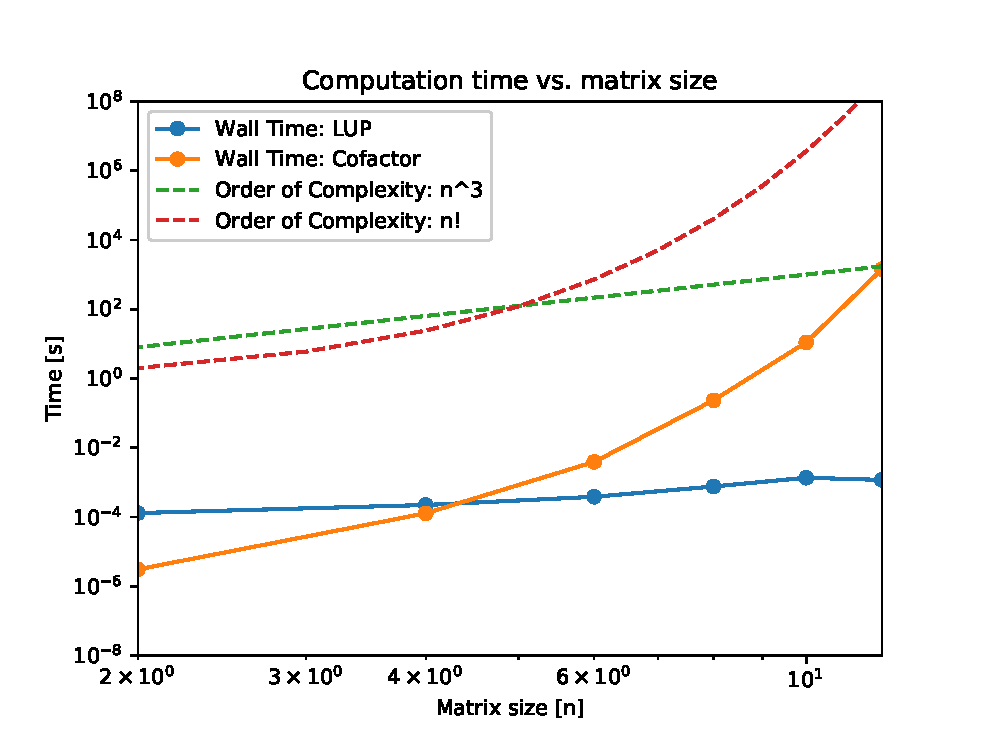
\includegraphics[width=0.75\textwidth]{figure/Figure_1.eps}
        \caption{Wall times vs. matrix size for the Cofactor expansion and LUP factorisation methods.}
        \label{fig:1}
  \end{figure}

For the purpose of analysis, the determinant values obtained through the two algorithms were compared with the results computed using \texttt{numpy} which uses the \texttt{LAPACK} subroutine \texttt{dgetrf}. The absolute error was then defined as $$e_{abs} = |\det(A)_{method} - \det(A)_{numpy}|$$ As shown in fig.~\ref{fig:2}, the absolute errors obtained through LUP factorisation were around 2 orders higher than the errors obtained through cofactor expansion. This can be attributed to the rounding errors during the LUP factorisation step. Since, cofactor matrix does not involve factorisation step, the errors due to factorisation due not arise and the errors in determinants are lower compared to LUP factorisation. However, the errors in both the cases were less than the order of precision of floating point numbers. The same arguments hold for the relative error which is defined as $$e_{rel} = \frac{|\det(A)_{method} - \det(A)_{numpy}|}{|\det(A)_{numpy}|}$$ The relative errors have been shown in fig.~\ref{fig:3}. It must be mentioned that due to the relatively small number of feasible computations, a notable error trend wasn't observed.
\begin{figure}[]
      \centering
      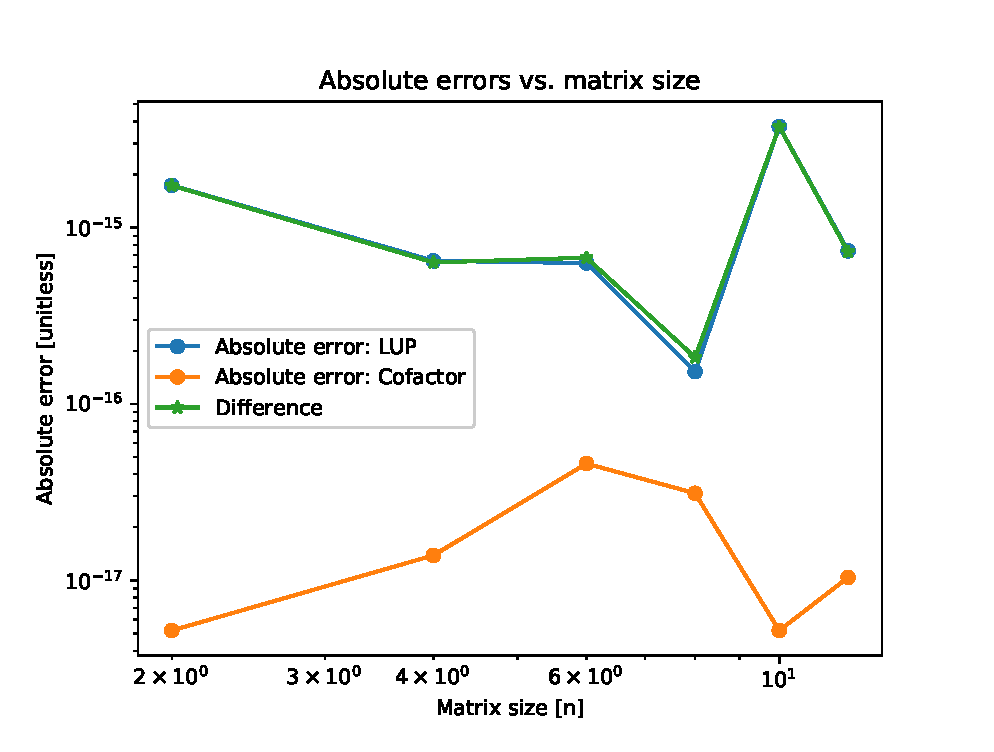
\includegraphics[width=0.75\textwidth]{figure/Figure_2.eps}
      \caption{Absolute error (w.r.t. \texttt{numpy})  vs. matrix size for the Cofactor expansion and LUP factorisation methods. The difference between the results from the two methods is also shown.}
      \label{fig:2}
\end{figure}
\begin{figure}[]
      \centering
      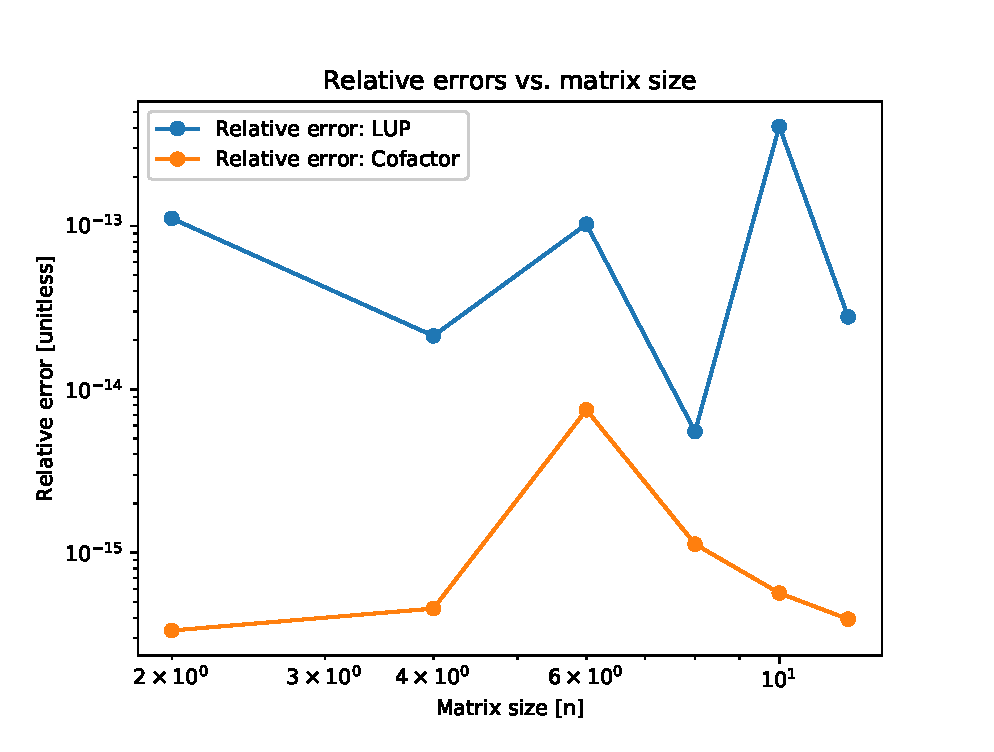
\includegraphics[width=0.75\textwidth]{figure/Figure_3.eps}
      \caption{Relative error (w.r.t. \texttt{numpy})  vs. matrix size for the Cofactor expansion and LUP factorisation methods.}
      \label{fig:3}
\end{figure}

\begin{figure}[]
      \centering
      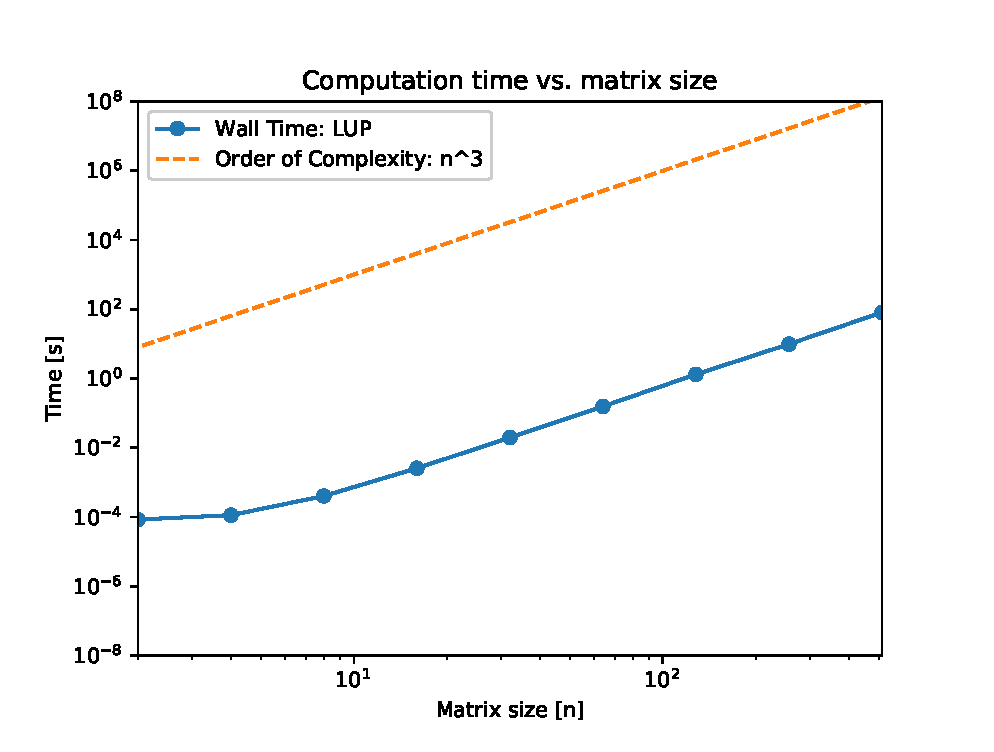
\includegraphics[width=0.75\textwidth]{figure/Figure_4.eps}
      \caption{Wall times vs. matrix size for the LUP factorisation method.}
      \label{fig:4}
\end{figure}
\begin{figure}[]
      \centering
      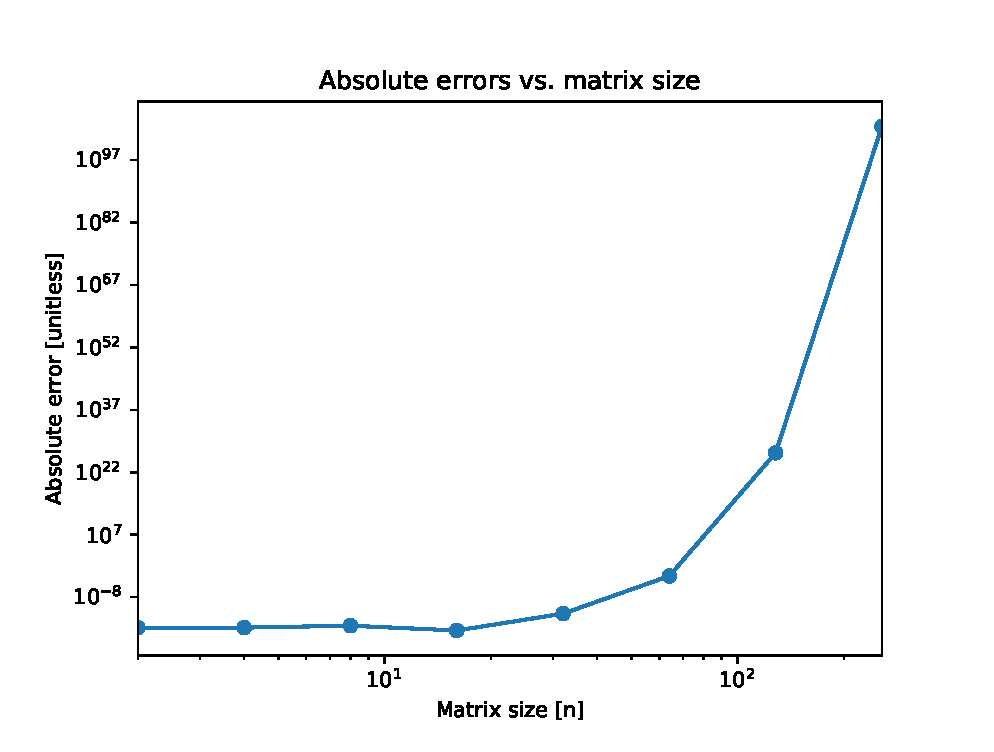
\includegraphics[width=0.75\textwidth]{figure/Figure_5.eps}
      \caption{Absolute error (w.r.t. \texttt{numpy})  vs. matrix size for the LUP factorisation method.}
      \label{fig:5}
\end{figure}
\begin{figure}[]
      \centering
      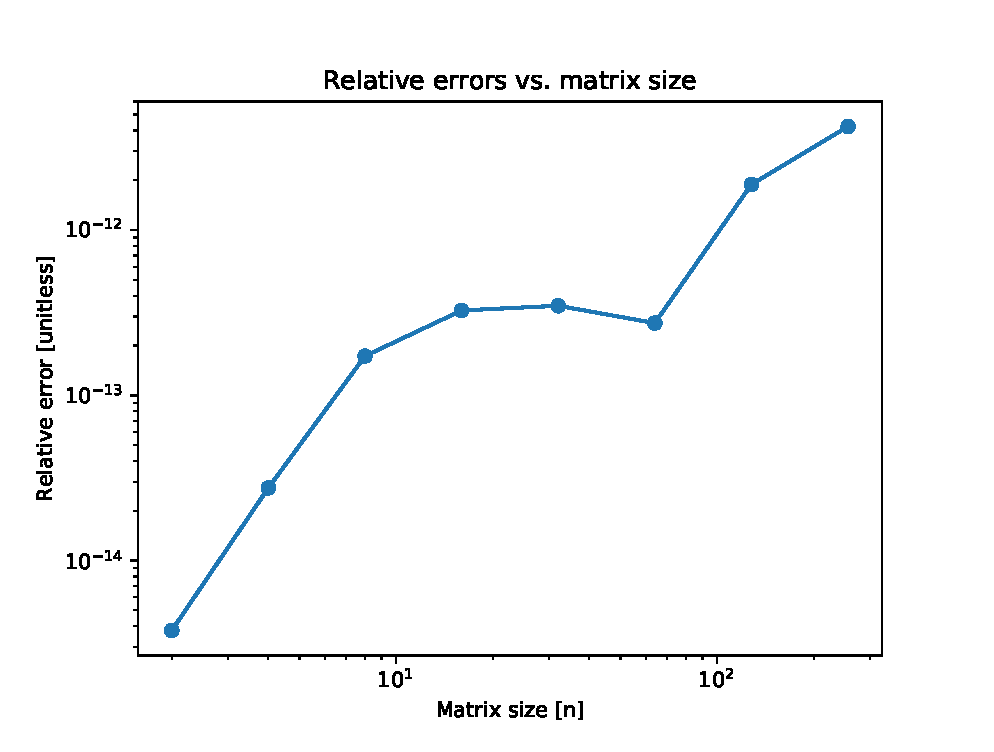
\includegraphics[width=0.75\textwidth]{figure/Figure_6.eps}
      \caption{Relative error (w.r.t. \texttt{numpy})  vs. matrix size for the LUP factorisation method.}
      \label{fig:6}
\end{figure}

The LUP factorisation method does not face the computational limitations observed in the cofactor expansion method and therefore the computations were performed for matrices of sizes upto $256\times256$. The results are shown in figs.\ref{fig:4}--\ref{fig:6}. The computation time follows the $\mathcal{O}(N^3)$ trend and the absolute error grows exponentially with matrix size.

\subsection*{Summary of results}
The order of complexity for the cofactor expansion method was demonstrated to be $\mathcal{O}(N!)$ while that for LUP factorisation was demonstrated to be $\mathcal{O}(N^3)$. As a result, LUP factorisation results in much faster calculation of the determinant of a matrix albeit at the cost of accuracy. However, the errors are well below the precision of floating point numbers which makes LUP factorisation computationally more efficient. The theoretically foreseen behaviour was observed in the computational results thus \textit{a-posteriori} verifying the theoretical proofs.
\end{document}
